\documentclass[12pt,letterpaper]{article}
\usepackage{amsmath,amsthm,amsfonts,amssymb,amscd}
\usepackage{fullpage}
\usepackage{lastpage}
\usepackage{enumerate}
\usepackage{fancyhdr}
\usepackage{mathrsfs}
\usepackage[margin=3cm,bottom=6cm]{geometry}
\usepackage{wrapfig}
\usepackage{graphicx}

\setlength{\parindent}{0.0in}
\setlength{\parskip}{0.05in}

\renewcommand{\theenumi}{\bf\Alph{enumi}}


% Edit these as appropriate
\newcommand\course{Math 227C}
\newcommand\semester{Spring 2019}     % <-- current semester
\newcommand\hwnum{1}                  % <-- homework number
\newcommand\yourname{Jun Allard} % <-- your name
%\newcommand\login{jcarberr}           % <-- your CS login

\newenvironment{answer}[1]{
  \subsubsection*{Problem \hwnum.#1}
}{\newpage}

\pagestyle{fancyplain}
\headheight 35pt
\lhead{ Math 227C }
\chead{\textbf{ Problem Set 2}}
%\rhead{Due {\bf Friday, April 13th}}
\headsep 20pt

\begin{document}


%\begin{enumerate}


%%%%%%%%%%%%%% PROBLEM %%%%%%%%%%%%%%%%%%
%\item
The DNA sequence of a gene determines the amino acid sequence of the protein it produces, with every 3 DNA basepairs coding for one protein amino acid. In eukaryotes, predicting the protein sequence from a gene sequence is not as simple as taking the gene sequence and splitting it into 3's, because of \emph{introns}, stretches of gene sequence that do not code for amino acids. (The regions of DNA in a gene that are not introns are called exons.)

A Markov chain model has been used to detect introns, assuming the 6 states shown in the diagram.
\begin{figure}[h!]
\centering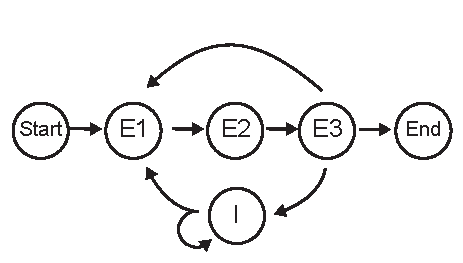
\includegraphics[width=8cm]{figP21}
\end{figure}

\begin{enumerate}[i]
\item Suppose a newly-discovered species has the following properties:
\begin{itemize}
\item The average protein-coding gene is $L_{\rm g} = 70000$ basepairs long.
\item The average protein-coding gene has $N_I=11$ introns.
\item The average intron is $L_I=6000$ basepairs long. 
\end{itemize}
Write the 6-state Markov transition matrix. The matrix should contain numerical values (e.g., expressed as a fraction or decimal). 
\item Under the assumptions of this model, what is the average length of a protein?
\end{enumerate}

%\end{enumerate}

\end{document}

%%%%%%%%%%%%%%%%%%%%%%%%%%%%%%%%%%%%%% 

